
\documentclass[a4paper]{scrreprt}
 
\usepackage[german]{babel}
\usepackage[utf8]{inputenc}
\usepackage[T1]{fontenc}
\usepackage{ae}

\usepackage[scaled]{helvet}
\renewcommand\familydefault{\sfdefault} 

\usepackage[onehalfspacing]{setspace}
\usepackage[scaled]{helvet}
\renewcommand*\familydefault{\sfdefault}

\usepackage[T1]{fontenc}
\usepackage{glossaries}
\usepackage{graphicx}
\usepackage[bookmarks,bookmarksnumbered]{hyperref}
\usepackage{float}
\usepackage[font={footnotesize}]{caption}

\setcounter{tocdepth}{1} 
\setcounter{secnumdepth}{2} 

\makenoidxglossaries

\newglossaryentry{Server}
{	name=Server,
	description={Ein Server (englisch server, wörtlich Diener oder Bediensteter, im weiteren Sinn auch Dienst) ist ein Computerprogramm oder ein Computer, der Computerfunktionalitäten wie Dienstprogramme, Daten oder andere Ressourcen bereitstellt, damit andere Computer oder Programme („Clients“) darauf zugreifen können}
}

\newglossaryentry{App}
{ 	name=App,
	plural=Apps,
	description={Als Mobile App (auf Deutsch meist in der Kurzform die App, eine Abkürzung für den Fachbegriff Applikation) wird eine Anwendungssoftware für Mobilgeräte beziehungsweise mobile Betriebssysteme bezeichnet}
}

\newglossaryentry{Nutzer}
{	name=Nutzer,
	description={Ein Benutzer (auch Endbenutzer, Bediener oder kurz Nutzer genannt sowie englisch User) ist eine Person, die ein Hilfs- oder Arbeitsmittel zur Erzielung eines Nutzens verwendet, beispielsweise für eine Zeitersparnis oder Kostensenkung}
}

\newglossaryentry{Desktop Anwendung}
{	name=Desktop Anwendung,
	plural=Desktop Anwendungen,
	description={Als Desktop Anwendungen (auch Anwendungsprogramm, kurz Anwendung oder Applikation; englisch application software, kurz App) werden Computerprogramme bezeichnet, die genutzt werden, um eine nützliche oder gewünschte nicht systemtechnische Funktionalität zu bearbeiten oder zu unterstützen. Sie dienen der „Lösung von Benutzerproblemen“}
}

\newglossaryentry{Drag and Drop}
{	name=Drag and Drop,
	description={Drag and Drop, oft auch Drag’n’Drop, deutsch „Ziehen und Ablegen“, ist eine Methode zur Bedienung grafischer Benutzeroberflächen von Rechnern durch das Bewegen grafischer Elemente mittels eines Zeigegerätes. Ein Element wie z. B. ein Piktogramm kann damit gezogen und über einem möglichen Ziel losgelassen werden. Dieses kann zum Beispiel markierter Text oder das Symbol einer Datei sein }
}

\newglossaryentry{Medikament}
{	name=Medikament,
	description={Arzneimittel oder gleichbedeutend Medikamente (lateinisch medicamentum „Heilmittel“) sind Stoffe oder Stoffzusammensetzungen, die „zur Heilung oder zur Verhütung menschlicher oder tierischer Krankheiten bestimmt sind“ oder sich dazu eignen, physiologische Funktionen zu beeinflussen oder eine medizinische Diagnose zu ermöglichen}
}

\newglossaryentry{NFC}
{ 	name=NFC,
	description={Die Nahfeldkommunikation (Near Field Communication, abgekürzt NFC) ist ein auf der RFID-Technik basierender internationaler Übertragungsstandard zum kontaktlosen Austausch von Daten per elektromagnetischer Induktion mittels loser gekoppelter Spulen über kurze Strecken von wenigen Zentimetern}
}

\newglossaryentry{Versichertennummer}
{ 	name=Versichertennummer,
	description={Die Krankenversichertennummer dient der Identifikation des Versicherten bei einer Krankenversicherung. Die Krankenversichertennummer wird benötigt, damit Leistungserbringer, z. B. Ärzte oder Zahnärzte ihre Leistungen mittels der Krankenversicherungskarte, über die Kassenärztlichen Vereinigungen, mit der zuständigen Krankenkasse abrechnen können}
}


\newglossaryentry{Bluetooth}
{	name=Bluetooth,
	description={Bluetooth ist ein in den 1990er Jahren durch die Bluetooth Special Interest Group (SIG) entwickelter Industriestandard gemäß IEEE 802.15.1 für die Datenübertragung zwischen Geräten über kurze Distanz per Funktechnik (WPAN). Dabei sind verbindungslose sowie verbindungsbehaftete Übertragungen von Punkt zu Punkt und Ad-hoc- oder Piconetze möglich}
}

\newglossaryentry{Pop-Up}
{	name=Pop-Up,
	description={Ein Pop-up (von englisch to pop up, „plötzlich auftauchen“) ist ein Element einer grafischen Benutzeroberfläche. In der Regel werden Pop-ups eingesetzt, um zusätzliche Inhalte anzuzeigen oder eine bestimmte Interaktion abzufragen. Typischerweise „springen“ Pop-ups auf und überdecken dabei andere Teile der Benutzeroberfläche}
}

\newglossaryentry{Cloud}
{	name=Cloud,
	description={Die Cloud ist keine physische Größe, sondern ein riesiges Netzwerk aus Remoteservern, die über die ganzen Welt verteilt aber miteinander verbunden sind, damit sie als ein einziges großes Ökosystem funktionieren können}
}

\newglossaryentry{Tab}
{	name=Tab,
	description={Eine Registerkarte, auch Reiter oder Tab genannt, ist ein Steuerelement einer grafischen Benutzeroberfläche, das einem Registerblatt aus Aktenschränken nachempfunden wurde }
}
 
\newglossaryentry{Arztbrief}
{	name=Arztbrief,
	plural=Arztbriefe,
	description={Der Arztbrief, oft synonym als Epikrise, Entlassungsbrief, Patientenbrief oder Befundbericht bezeichnet, ist ein Transferdokument für die Kommunikation zwischen Ärzten. Der Arztbrief gibt einen zusammenfassenden Überblick über den Status des Patienten bei der Entlassung, einen Rückblick über den Krankheitsverlauf, die veranlasste Therapie, eine Interpretation des Geschehens zum Krankheitsverlauf im speziellen Fall}
}

\newglossaryentry{Anamnese}
{	name=Anamnese,
	description={Die Anamnese (von altgriechisch anámnēsis, deutsch ‚Erinnerung‘) ist die professionelle Erfragung von potenziell medizinisch relevanten Informationen durch Fachpersonal (z. B. einen Arzt)}
}
 
\begin{document}
\begin{titlepage}
\begin{figure}[h]
	\vspace{-4cm}
	\hspace{-2cm}
	
\includegraphics[ width=0.3\textwidth]{Kit_Logo}
	\label{fig:Aufg03_1}
\end{figure}
	\vspace{1.5cm}
	\centering
	
\includegraphics[width=0.5\textwidth]{graphics/myMD_Logo}\par\vspace{0.5cm}
	{\Huge myMD \par}
	\vspace{2cm}
	{\scshape\Large Qualitätssicherung\par}
	\vspace{1cm}
	Praxis der Softwareentwicklung WS2017/2018 \par
	\vspace{2cm}
	{\Large\itshape Philipp Pelcz, Philipp Karcher, Jan-Luca Vettel\par}
	\vfill
	supervised by \par
	Marc Aurel Kiefer

	\vfill

% Bottom of the page
	{\large \today \par}
\end{titlepage}
 

% Platzierung des Inhaltsverzeichnisses
\tableofcontents
\addtocontents{toc}{\protect\enlargethispage{10cm}}

\chapter{Einleitung}
\dq{}myMD\dq{} ist eine mobile Anwendung, die es Patienten erlaubt, ihre Arztbriefe digital über Bluetooth von ihren Ärzten zu erhalten, um dann in der Applikation die darin enthaltenen Informationen, wie die Diagnose oder verschrieben Medikationen, einsehen zu können. \newline
\newline
Die App wurde dabei mit Xamarin.Forms in C\# und XAML für Android- und iOS-Geräte entwickelt. 
\newline
\newline
Aufbauend auf den Tests, die im Pflichtenheft aufgestellt wurden, haben wir in der Phase der Qualitätssicherung unsere App auf Fehler überprüft. Dazu haben wir viele Unit-KomponentenTests geschrieben, aber auch manche Funktionen, für die Unit-Tests ungeeignet sind, manuell getestet.
\newline
\newline
In diesem Dokument werden diese Tests aufgeführt und kurz beschrieben. Außerdem werden auch nennenswerte Fehler und ihre Lösung kurz beschrieben.
\chapter{Testvorbereitung}
\section{Zu testende Komponenten}
Da sich unser System aus drei Subsystemen (\textbf{Model}, \textbf{ViewModel}, \textbf{View}) zusammensetzt, sollten alle drei Subsysteme getestet werden. Jedoch lässt sich die \textbf{View} nicht automatisch testen, da sie nur die Benutzeroberfläche und ihre Logik enthält. Außerdem ist sie sehr stark mit dem \textbf{ViewModel} verknüpft. Deshalb haben wir uns entschieden, das \textbf{ViewModel} und die \textbf{View} zusammen zu testen. Dadurch ergeben sich die UnitTests für das \textbf{Model} und die UITests für das \textbf{ViewModel} und die \textbf{View}.

\section{Testvorgaben aus dem Pflichtenheft}
Im folgenden werden alle Systemtests aus dem Pflichtenheft mit ihren Ergebnissen aufgeführt. Da manche Tests (vorallem Datenübertragungs- und Übersicht-Tests) eine Bluetoothübertragung benötigen konnten diese nicht vollständig automatisch durchgeführt werden. Denn das emulierte Testhandy bietet keine Möglichkeit einer Bluetoothdatenübertragung. Diese Tests wurden manuell getestet. Außerdem bietet Xamarin.Forms keine Möglichkeit UITests (Systemtests) für ein UWP an. Deshalb wurden die alle Tests, die die Desktop-Anwendung betreffen, auch manuell durchgeführt. Da wir uns bei der Implementierung an den, im Pflichtenheft vorgegebenen, Tests entlanggehangelt haben, laufen diese Tests fehlerfrei.\newline \newline
\textit{Legende:} \newline
A[BT0000]  $\widehat{=}$ Test \dq{}BT000\dq{} wurde automatisch durchgeführt \newline
M[BT0000]  $\widehat{=}$ Test \dq{}BT000\dq{} wurde manuell durchgeführt \newline
E[BT0000]  $\widehat{=}$ Die Funktion, die den Test \dq{}BT000\dq{} benötigt wurde entfernt, nicht implementiert oder modifiziert
\subsection{Basis Testfälle (BT)}
\subsubsection{Patientenseitige Datenübertragung}
\begin{tabular}{lll}
M[BT1010] & \multicolumn{2}{p{12cm}}  {\gls{Desktop Anwendung} sendet eine Datei an die myMD \gls{App}.} \\
{E[BT1020]} & \multicolumn{2}{p{12cm}}  {Die Übertragung wird vom \gls{Nutzer} unterbrochen.} \\
{M[BT1030]} & \multicolumn{2}{p{12cm}}  {\gls{Desktop Anwendung} sendet eine unzulässige Datei (nicht unterstütztes Dateiformat).} \\
{M[BT1040]} & \multicolumn{2}{p{12cm}}  {Die Übertragung wird durch äußere Umstände abgebrochen.} \\

\end{tabular}

\subsubsection{Darstellung}
\begin{tabular}{lll}
M[BT2010] & \multicolumn{2}{p{12cm}}  {Ein neuer \gls{Arztbrief} wird in eine leere Übersicht geladen.} \\
{M[BT2020]} & \multicolumn{2}{p{12cm}}  {Ein neuer \gls{Arztbrief} wird in bereits gefüllte Übersicht geladen.} \\
{M[BT2030]} & \multicolumn{2}{p{12cm}}  {Ein digitaler \gls{Arztbrief} wird angetippt/geöffnet.} \\
{M[BT2040]} & \multicolumn{2}{p{12cm}}  {Ein digitaler \gls{Arztbrief} wird geschlossen.} \\
{M[BT2050]} & \multicolumn{2}{p{12cm}}  {Ein digitaler \gls{Arztbrief} wird gelöscht.} \\

\end{tabular}

\subsubsection{Einstellungen}
\begin{tabular}{lll}
{A[BT3010]} & \multicolumn{2}{p{12cm}}  {Das Nutzerprofil wird bearbeitet.} \\
\end{tabular}

\subsubsection{\gls{Desktop Anwendung}}
\begin{tabular}{lll}
{M[BT4010]} & \multicolumn{2}{p{12cm}}  {Unzulässige Datei wird zum Senden ausgewählt.} \\
{M[BT4020]} & \multicolumn{2}{p{12cm}}  {Kompatible Datei wird zum Senden ausgewählt.} \\
{M[BT4030]} & \multicolumn{2}{p{12cm}}  {Senden wird erfolgreich abgeschlossen.} \\
{M[BT4040]} & \multicolumn{2}{p{12cm}}  {Senden wird durch äußere Einflüsse unterbrochen.} \\
{M[BT4050]} & \multicolumn{2}{p{12cm}}  {Senden wird durch \gls{Nutzer} unterbrochen.} \\
{E[BT4060]} & \multicolumn{2}{p{12cm}}  {Geräte in der Nähe werden gesucht.} \\
{E[BT4070]} & \multicolumn{2}{p{12cm}}  {Nutzergerät wird als Empfänger gewählt.} \\



\end{tabular}

\subsection{Erweiterte Testfälle (ET)}
\subsubsection{Patientenseitige Datenübertragung}
\begin{tabular}{lll}
E[ET1010] & \multicolumn{2}{p{12cm}}  {myMD \gls{App} sendet eine Datei an die \gls{Desktop Anwendung}.} \\
{E[ET1020]} & \multicolumn{2}{p{12cm}}  {myMD \gls{App} sendet mehrere Dateien an die \gls{Desktop Anwendung}.} \\
{M[ET1030]} & \multicolumn{2}{p{12cm}}  {\gls{Desktop Anwendung} sendet mehrere Datei an die myMD \gls{App}.} \\
{M[ET1040]} & \multicolumn{2}{p{12cm}}  {Die Übertragung mehrerer Daten wird durch äußere Umstände abgebrochen.} \\
{M[ET1050]} & \multicolumn{2}{p{12cm}}  {Die Übertragung mehrerer Daten wird durch den \gls{Nutzer} abgebrochen.} \\
{E[ET1060]} & \multicolumn{2}{p{12cm}}  {Sensible Daten werden von der myMD \gls{App} an die \gls{Desktop Anwendung} gesendet.} \\
{E[ET1070]} & \multicolumn{2}{p{12cm}}  {Die Verbindung wird über NFC hergetellt.} \\
{E[ET1080]} & \multicolumn{2}{p{12cm}}  {Ein Profil wird auf ein anderes Gerät übertragen.} \\

\end{tabular}

\subsubsection{Darstellung}
\begin{tabular}{lll}
A[ET2010] & \multicolumn{2}{p{12cm}}  {\gls{Medikament} wird hinzugefügt.} \\
{A[ET2020]} & \multicolumn{2}{p{12cm}}  {\gls{Medikament} wird editiert.} \\
{A[ET2030]} & \multicolumn{2}{p{12cm}}  {\gls{Medikament} wird gelöscht.} \\
{E[ET2040]} & \multicolumn{2}{p{12cm}}  {Laborwerte werden hinzugefügt.} \\
{E[ET2050]} & \multicolumn{2}{p{12cm}}  {Laborwerte werden gelöscht.} \\{E[ET2060]} & \multicolumn{2}{p{12cm}}  {Bilddatei wird hinzugefügt und dargestellt.} \\
{E[ET2070]} & \multicolumn{2}{p{12cm}}  {Bilddatei wird mit einem \gls{Arztbrief} verknüpft.} \\
{E[ET2080]} & \multicolumn{2}{p{12cm}}  {Verknüpfung zwischen \gls{Arztbrief} und Bilddatei wird getrennt.} \\
{E[ET2090]} & \multicolumn{2}{p{12cm}}  {Überprüfung, ob eine Bilddatei originalgetreu ist.} \\
{E[ET2100]} & \multicolumn{2}{p{12cm}}  {Mehrere \glspl{Arztbrief} gruppieren.} \\
{E[ET2110]} & \multicolumn{2}{p{12cm}}  {Einzelne \glspl{Arztbrief} aus bestehender Gruppe entfernen.} \\
{E[ET2120]} & \multicolumn{2}{p{12cm}}  {Nach eigenen Gruppen sortieren.} \\
{E[ET2130]} & \multicolumn{2}{p{12cm}}  {Überprüfen, ob Suchfunktion fehlerfrei funktioniert.} \\


\end{tabular}

\subsubsection{Einstellungen}
\begin{tabular}{lll}
A[ET3010] & \multicolumn{2}{p{12cm}}  {Neues Nutzerprofil wird angelegt.} \\
{E[ET3020]} & \multicolumn{2}{p{12cm}}  {Ein weiteres Nutzerprofil wird angelegt.} \\
{E[ET3030]} & \multicolumn{2}{p{12cm}}  {Ein Nutzerprofil wird gelöscht.} \\
{E[ET3040]} & \multicolumn{2}{p{12cm}}  {Wechsel zwischen mehreren Nutzerprofilen.} \\
{E[ET3050]} & \multicolumn{2}{p{12cm}}  {Einzelnen \gls{Arztbrief} als sensibel markieren.} \\
{E[ET3060]} & \multicolumn{2}{p{12cm}}  {Sensibiltäts-Markierung eines einzelnen Arztbriefes aufheben.} \\
{E[ET3070]} & \multicolumn{2}{p{12cm}}  {Gruppe von Arztbriefen als sensibel markieren.} \\
{E[ET3080]} & \multicolumn{2}{p{12cm}}  {Sensibiltäts-Markierung einer Gruppe von Arztbriefen aufheben.} \\
{E[ET3090]} & \multicolumn{2}{p{12cm}}  {Regelmäßiger Arzttermin wird hinzugefügt.} \\
{E[ET3100]} & \multicolumn{2}{p{12cm}}  {Regelmäßiger Arzttermin wird gelöscht.} \\

\end{tabular}

\subsubsection{\gls{Desktop Anwendung}}
\begin{tabular}{lll}
{E[ET4010]} & \multicolumn{2}{p{12cm}}  {Datei mit falscher Versichertennummer wird gesendet.} \\


\end{tabular}

\chapter{Automatische Tests}

\section{Unit Tests}
\subsection{DatabaseModel}
\subsubsection{EntityDatabase}
\begin{tabular}{lll}
{GetDataFromProfileTest} & \multicolumn{2}{p{12cm}}  {Überprüfung, ob die Daten eines Profils korrekt gespeichert werden.} \\
{DLetterGroupDLetter} & \multicolumn{2}{p{12cm}}  {Überprüfung, ob Arztbriefe korrekt gruppiert werden können.} \\
{EqualTest} & \multicolumn{2}{p{12cm}}  {Überprüfung, ob zwei Arztbriefgruppen gleich sind.} \\
{DeleteTest} & \multicolumn{2}{p{12cm}}  {Überprüfung, ob ein Arztbrief korrekt gelöscht wird.} \\
{GetDoctorTest} & \multicolumn{2}{p{12cm}}  {Überprüfung, der Arzt innerhalb eines Arztbriefes korrekt zurückgegeben wird.} \\
{GetProfilTest} &
\multicolumn{2}{p{12cm}}  {Überprüfung, ein Profil aus der Datenbank korrekt \newline zurückgegeben wird.} \\
\end{tabular}
\subsubsection{Database}
\begin{tabular}{lll}
{MedLetterTest} & \multicolumn{2}{p{12cm}}  {Überprüfung, ob eine Medikation mit einem Arztbrief verknüpft werden kann} \\
{GroupTest} & \multicolumn{2}{p{12cm}}  {Überprüfung, ob Arztbriefe mit verknüpften Medikationen gruppiert werden können.} \\
\end{tabular}

\subsection{DataModel}
\subsubsection{MedicationTest}
\begin{tabular}{lll}
{SameEqualTest} & \multicolumn{2}{p{12cm}}  {Überprüfung, ob die Überprüfung der Gleichheit zweier Medikamente korrekt ist.} \\
{CopiedEqualTest} & \multicolumn{2}{p{12cm}}  {Überprüfung, ob die Überprüfung der Gleichheit einer dublizierten Medikation korrekt ist.} \\
{NullEqualtest} & \multicolumn{2}{p{12cm}}  {Überprüfung, ob der Vergleich einer Medikation mit \textit{null} korrekt ist.} \\
{NotEqualTest} & \multicolumn{2}{p{12cm}}  {Überprüfung, ob die Überprüfung zweier ungleicher Medikamente auf Gleichheit korrekt ist.} \\
{LetterTest} & \multicolumn{2}{p{12cm}}  {Überprüfung, ob eine Medikation korrekt mit einem Arztbrief verknüpft wird.} \\
{DeleteTest} & \multicolumn{2}{p{12cm}}  {Überprüfung, ob eine Medikation, die mit einem Arztbrief verknüpft ist, korrekt gelöscht wird.} \\
\end{tabular}
\subsubsection{DoctorTest}
\begin{tabular}{lll}
{SameEqualTest} & \multicolumn{2}{p{12cm}}  {Überprüfung, ob die Überprüfung der Gleichheit zweier Ärzte korrekt ist.} \\
{CopiedEqualTest} & \multicolumn{2}{p{12cm}}  {Überprüfung, ob die Überprüfung der Gleichheit von dublizierten Ärzte korrekt ist.} \\
{NullEqualtest} & \multicolumn{2}{p{12cm}}  {Überprüfung, ob der Vergleich eines Arztes mit \textit{null} korrekt ist.} \\
{NotEqualTest} & \multicolumn{2}{p{12cm}}  {Überprüfung, ob die Überprüfung zweier ungleicher Ärzte auf Gleichheit korrekt ist.} \\
{IDoctorToDoctor} & \multicolumn{2}{p{12cm}}  {Überprüfung, ob ein \textit{IDoctor}-Objekt korrekt zu einem \textit{Doctor}-Objekt konvertiert wird.} \\
\end{tabular}
\subsubsection{DoctorTest}
\begin{tabular}{lll}
{SameEqualTest} & \multicolumn{2}{p{12cm}}  {Überprüfung, ob die Überprüfung der Gleichheit zweier Ärzte korrekt ist.} \\
{CopiedEqualTest} & \multicolumn{2}{p{12cm}}  {Überprüfung, ob die Überprüfung der Gleichheit von dublizierten Ärzten korrekt ist.} \\
{NullEqualtest} & \multicolumn{2}{p{12cm}}  {Überprüfung, ob der Vergleich eines Arztes mit \textit{null} korrekt ist.} \\
{NotEqualTest} & \multicolumn{2}{p{12cm}}  {Überprüfung, ob die Überprüfung zweier ungleicher Ärzte auf Gleichheit korrekt ist.} \\
{IDoctorToDoctor} & \multicolumn{2}{p{12cm}}  {Überprüfung, ob ein \textit{IDoctor}-Objekt korrekt zu einem \textit{Doctor}-Objekt konvertiert wird.} \\
\end{tabular}
\subsubsection{DoctorsLetterTest}
\begin{tabular}{lll}
{SameEqualTest} & \multicolumn{2}{p{12cm}}  {Überprüfung, ob die Überprüfung der Gleichheit zweier Arztbriefe korrekt ist.} \\
{CopiedEqualTest} & \multicolumn{2}{p{12cm}}  {Überprüfung, ob die Überprüfung der Gleichheit von dublizierten Arztbriefen korrekt ist.} \\
{NullEqualtest} & \multicolumn{2}{p{12cm}}  {Überprüfung, ob der Vergleich eines Arztbriefes mit \textit{null} korrekt ist.} \\
{NotEqualTest} & \multicolumn{2}{p{12cm}}  {Überprüfung, ob die Überprüfung zweier ungleicher Arztbriefe auf Gleichheit korrekt ist.} \\
{DeleteTest} & \multicolumn{2}{p{12cm}}  {Überprüfung, ob Arztbrief korrekt gelöscht wird.} \\
{MedicationTest} & \multicolumn{2}{p{12cm}}  {Überprüfung, ob Arztbrief verknüpfte Medikationen korrekt behandelt.} \\
{GroupTest} & \multicolumn{2}{p{12cm}}  {Überprüfung, ob sich Arztbriefe korrekt gruppieren lassen.} \\
\end{tabular}
\subsubsection{DoctorsLetterGroupTest}
\begin{tabular}{lll}
{DateTest} & \multicolumn{2}{p{12cm}}  {Überprüfung, ob eine Gruppe von Arztbriefen, richtige Daten behält.} \\
{AddTest} & \multicolumn{2}{p{12cm}}  {Überprüfung, ob eine Gruppe von Arztbriefen korrekt zu der Datenbank hinzugefügt wird.} \\
{CompareLetterTest} & \multicolumn{2}{p{12cm}}  {Überprüfung, ob die Überprüfung zweier gleicher Arztbriefgruppen korrekt funktioniert.} \\
{FirstLastDateTest} & \multicolumn{2}{p{12cm}}  {Überprüfung, ob die das früheste und das späteste Datum einer Arztbriefgruppe korrekt erkannt wird.} \\
{DeleteTest} & \multicolumn{2}{p{12cm}}  {Überprüfung, ob eine Arztbriefgruppe korrekt gelöscht wird.} \\
\end{tabular}
\subsection{FileHelper}
\begin{tabular}{lll}
{WriteFromBytesTest} & \multicolumn{2}{p{12cm}}  {Überprüfung, ob eine Datei korrekt in die Datenbank geschrieben wird.} \\
\end{tabular}
\subsection{ModelFacadeTest}
\begin{tabular}{lll}
{ProfileTest} & \multicolumn{2}{p{12cm}}  {Überprüfung, ob ein Profil korrekt aktiviert wird.} \\
{MedicationTest} & \multicolumn{2}{p{12cm}}  {Überprüfung, ob alle Medikationen von der Fassade zurückgegeben werden.} \\
{GroupTest} & \multicolumn{2}{p{12cm}}  {Überprüfung, ob alle Gruppen von Arztbriefen zurückgegeben werden.} \\
{UpdateTest} & \multicolumn{2}{p{12cm}}  {Überprüfung, ob die Fassade die Gruppen von Arztbriefen korrekt aktualisiert.} \\
{DeleteTest} & \multicolumn{2}{p{12cm}}  {Überprüfung, ob die Fassade eine Medikation korrekt löscht.} \\
\end{tabular}
\subsection{Parser}
\subsubsection{ParserFacadeTest}
\begin{tabular}{lll}
{ParseLetterToFile} & \multicolumn{2}{p{12cm}}  {Überprüfung, ob eine Datei korrekt in das ursprüngliche Dateiformat geschrieben wird.} \\
{ParseFileToDB} & \multicolumn{2}{p{12cm}}  {Überprüfung, ob eine Datei korrekt in die Datenbank geparsed wird.} \\
{ParseInvalidFile} & \multicolumn{2}{p{12cm}}  {Überprüfung, ob der Parser eine fehlerhafte Datei korrekt behandelt.} \\
\end{tabular}
\subsubsection{HL7ParserTest}
\begin{tabular}{lll}
{ParseFromDocument} & \multicolumn{2}{p{12cm}}  {Überprüfung, ob eine .hl7 Datei korrekt in die Datenbank geschrieben wird.} \\
{ParseSample} & \multicolumn{2}{p{12cm}}  {Überprüfung, ob eine Datei korrekt geparsed wird.} \\
{ParseHL7File} & \multicolumn{2}{p{12cm}}  {Überprüfung, ob eine .hl7 Datei korrekt in die Datenbank geschrieben wird.} \\
{ParseLetterToFile} & \multicolumn{2}{p{12cm}}  {Überprüfung, ob eine .hl7 Datei korrekt in das ursprüngliche Dateiformat geschrieben wird.} \\
{UnsupportedFile} & \multicolumn{2}{p{12cm}}  {Überprüfung, ob der Parser eine nichtunterstützte Datei korrekt behandelt.} \\
{InvalidFile} & \multicolumn{2}{p{12cm}}  {Überprüfung, ob der Parser eine fehlerhafte Datei korrekt behandelt.} \\
\end{tabular}
\subsubsection{FileToDatabaseParser}
\begin{tabular}{lll}
{ParseFileTest} & \multicolumn{2}{p{12cm}}  {Überprüfung, ob eine Datei korrekt in die Datenbank geschrieben wird.} \\
\end{tabular}
\subsection{TransmissionModel}
\begin{tabular}{lll}
{ListToArrayTest} & \multicolumn{2}{p{12cm}}  {Überprüfung, ob eine Liste an Byte-Arrays korrekt zu einer Datei zusammengesetzt wird.} \\
{EmptyListToArrayTest} & \multicolumn{2}{p{12cm}}  {Überprüfung, ob eine leere Liste an Byte-Arrays korrekt zu einer Datei zusammengesetzt wird.} \\
{GetNumberOfFilesTest} & \multicolumn{2}{p{12cm}}  {Überprüfung, ob die Anzahl der zu empfangenen Dateien korrekt ausgelesen wird.} \\
{GetReadCycles} & \multicolumn{2}{p{12cm}}  {Überprüfung, ob die Anzahl der Lesezyklen zu einer Datei korrekt ausgelesen wird.} \\
\end{tabular}
\section{UITests}
Die folgenden Tests werden mit Hilfe der UITests von Xamarin.Forms realisiert. Da diese auf einem emuliertem Handy, auf dem die ausführbare Datei der App läuft, getestet werden, können von diesen Tests keine Codeüberdeckung o.Ä. ermittelt werden.
\subsection{OverviewUITest}
\begin{tabular}{lll}
{AppLaunches} & \multicolumn{2}{p{12cm}}  {Überprüfung, ob die App korrekt startet.} \\
{EveryElement} & \multicolumn{2}{p{12cm}}  {Überprüfung, ob jedes Element der View vorhanden ist.} \\
\end{tabular}
\subsection{MedicationUITest}
\begin{tabular}{lll}
{CreateNewMed} & \multicolumn{2}{p{12cm}}  {Überprüfung, ob die View/ViewModel das erstellen einer neuen Medikation korrekt durchführt.} \\
{DeleteMed} & \multicolumn{2}{p{12cm}}  {Überprüfung, ob die View/ViewModel eine Medikation korrekt löscht.} \\
{EditMed} & \multicolumn{2}{p{12cm}}  {Überprüfung, ob die View/ViewModel eine Medikation korrekt editiert.} \\
\end{tabular}
\subsection{SendDataUITests}
\begin{tabular}{lll}
{AllButtonsThere} & \multicolumn{2}{p{12cm}}  {Überprüfung, ob alle Elemente des SendenTabs existieren.} \\
\end{tabular}
\subsection{ProfilUITests}
\begin{tabular}{lll}
{CreateNewProfil} & \multicolumn{2}{p{12cm}}  {Überprüfung, ob ein neues Profil korrekt erstellt wird.} \\
{EditProfil} & \multicolumn{2}{p{12cm}}  {Überprüfung, ob ein Profil korrekt editiert wird.} \\
\end{tabular}
\chapter{Manuelle Tests}
\section{Testszenarien}
Anhand der im Pflichtenheft erörterten Testszenarien haben wir die Testszenarien, dessen Funktionen wir auch umgesetzt haben,erfolgreich durchgeführt.
\subsection{Typischer Arztbesuch}
Der \gls{Nutzer} geht wegen einer Beschwerde zum Arzt und lässt sich untersuchen. Sobald die Untersuchung fertig ist, verlangt der \gls{Nutzer}, dass der Arzt ihm die eben aufgenommenen Daten für die myMD \gls{App} zur Verfügung stellt. Der Arzt öffnet dann die \gls{Desktop Anwendung} und schickt dem Patienten den \gls{Arztbrief} auf die myMD \gls{App}. Der \gls{Nutzer} schaut sich dann kurz den neuen Eintrag in der Übersicht an, schließt die App und geht nach Hause. \newline

\begin{tabular}{lll}
[BT4060] & \multicolumn{2}{p{12cm}}  {Geräte in der Nähe werden gesucht.} \\
{[BT4070]} & \multicolumn{2}{p{12cm}}  {Das Mobilgerät des Nutzers wird als Empfänger ausgewählt.} \\
{[BT4030]} & \multicolumn{2}{p{12cm}}  {Senden wird erfolgreich abgeschlossen.} \\
{[BT2020]} & \multicolumn{2}{p{12cm}}  {Der neue \gls{Arztbrief} wird in bereits gefüllte Übersicht geladen.} \\
{[BT2030]} & \multicolumn{2}{p{12cm}}  {Der neue \gls{Arztbrief} wird geöffnet.} \\
{[BT2040]} & \multicolumn{2}{p{12cm}}  {Der neue \gls{Arztbrief} wird geschlossen.} \\


\end{tabular}

\subsection{Krankenhistorie wird überprüft}
Der \gls{Nutzer} ist daheim und schaut sich in der myMD \gls{App} seine Übersicht an. Er klickt auf einige \glspl{Arztbrief} und liest sich durch, was darin steht. Dann bemerkt er, dass er die verschriebenen Medikamente zu seinem gebrochenen Fuß  in den \gls{Tab} \textit{\gls{Medikament}e} hinzufügen sollte. Versehentlich gibt er zuerst eine falsche Menge an, korrigiert diese aber und schließt daraufhin die App.\newline

\begin{tabular}{lll}
[BT2030] & \multicolumn{2}{p{12cm}}  {Ein \gls{Arztbrief} wird geöffnet.} \\
{[BT2040]} & \multicolumn{2}{p{12cm}}  {Ein \gls{Arztbrief} wird geschlossen.} \\
{[ET2010]} & \multicolumn{2}{p{12cm}}  {\gls{Medikament} wird hinzugefügt.} \\
{[ET2020]} & \multicolumn{2}{p{12cm}}  {\gls{Medikament} wird editiert.} \\

\end{tabular}

\section{Desktop-Anwendung}
Das automatische Testen der Desktop-Anwendung hat sich als sehr schwierig herausgestellt, da die Unterstützung von Unit-Tests einer UWP-Anwendung nur sehr dürftig ausfällt. Die oben beschriebenen UITests, die für die App benutzt wurden, werden für eine UWP-Anwendung sogar überhaupt nicht angeboten. Um dennoch eine möglichst fehlerfreie Funktionsweise der Anwendung gewährleisten zu können, wurde diese ausgiebig manuell getestet. Da zugleich der Funktionsumfang der Desktop-Anwendung nur gering ausfällt, war dies eine legitime Vorgehensweise.
\chapter{Verbleibende Bugs}
\begin{tabular}{p{12cm} |l| }
\textbf{Beschreibung} & \textbf{Priorität} \\
Der Server auf der Desktop-Anwendung wird nicht gestoppt. & Mittel \\
Durch den physischen Zurück-Button lassen sich leere Medikamente erstellen. & Mittel \\
Server ist manchmal nicht entdeckbar, falls er über eine längere Zeit (>15 Minuten) läuft. & Hoch \\
Durch schnelles Klicken lassen sich manche Pages mehrmals öffnen. & Niedrig \\
Die App stürzt ab, wenn man mit einem Gerät ohne Bluetooth (z.B. Emulator) nach Geräten sucht. & Hoch \\
Die App schließt sich unerwartet, wenn man während dem Geräte suchen das Bluetooth deaktiviert.Leider konnten wir diesen Bug noch nicht reproduzieren. & Mittel

\end{tabular}
\chapter{Interessante Bugs und ihre Lösung}
\textbf{Beschreibung:} Beim ersten Start der App ist die App abgestürzt. Dies lag daran, dass die App ein aktives Profil benötigt um eine Entität (hier: ein neues leeres Profil) der Datenbank hinzuzufügen. Da zum ersten Start jedoch noch kein Profil existierte stürzte die App ab.
\textbf{Lösung:} Das neue Profil wird zuerst erstellt aktiviert bevor es in die Datenbank eingefügt wird. \newline \newline
\textbf{Beschreibung:} Das Löschen einer Datei war nicht möglich, da einem die Zugriffsrechte auf die Datei verweigert wurden. \newline
\textbf{Lösung:} Es wurde nichtmehr der komplette Dateipfad, sondern der lokale Teilpfad gespeichert. \newline \newline
\textbf{Beschreibung:} Die App ist beim Öffnen des \textit{SendDataTabs} abgestürzt, da wir im Konstruktor auf den \textit{BluetoothAdapter} zugegriffen haben. Jedoch war zu diesem Zeitpunkt der Kontext noch nicht verfügbar. \newline
\textbf{Lösung:} Der Adapter wird nichtmehr im Konstruktor eines \textit{ViewModels} aufgerufen, sondern immer nur durch einen \textit{ButtonClick} \newline \newline
\textbf{Beschreibung: }Die App lässt sich nichtmehr kompilieren, da der Linker sich über zu große Dateien beschwert. Die zu große Datei war das \textit{Everest-Framework}, welches wir zum Parsen der empfangenen Datei nutzten. Da dieses Framework viele generische Datentypen nutzte und auch anbot, wuchs die Dateigröße beim compilieren enorm.\newline
\textbf{Lösung: }Das \textit{Everest-Framework} wurde aus dem Projekt geschmissen und wir schrieben unseren eigenen Parser. \newline \newline
\textbf{Beschreibung:} Es ließ sich auf dem Handy kein \textit{GATT-Server} zur Datenübertragung erstellen. Dies lag daran, dass das Handy den \textit{Bluetooth-State} als \dq{}UNKNOWN\dq{} erkannte, obwohl dieser \dq{}POWERED-ON\dq{} sein sollte. Dies war ein Bug aus dem Bluetooth-Framework, welches wir für die Datenübertragung nutzten. \newline
\textbf{Lösung:} Der \textit{GATT-Server} wird nun auf der Desktop-Anwendung gestartet und die App ließt die benötigten Dateien aus der Dektop-Anwendung. \newline \newline
\textbf{Beschreibung: }Wir wollten gefundene Geräte nur einmal in der Liste darstellen und haben dafür das Attribut ListRepeatedBroadcast auf false gesetzt. Dadurch wurde ein Gerät aber für diese ServerSession nur noch einmal angezeigt. Dies war ein Problem, falls man längere Sessions geführt hat oder erneut nach verfügbaren Geräten gesucht hat \newline
\textbf{Lösung:} Wir haben das oben genannte Attribut auf true gesetzt und unsere eigene Logik für das mehrmalige Aufzählen von dem gleichen Gerät implementiert.
\chapter{Anhang}
\section{Nutzerstudie}
Diese Nutzerstudie soll uns Informationen über die Nutzerfreundlichkeit geben. Dabei wurde jedem Tester gesagt welche Aktion er ausführen soll und wir dokumentierten den Erfolg über diese Aktionen.
\textit{Hinweis: Nicht alle Tests konnten von allen Testern durchgeführt werden, da nicht alle Tester Zugriff auf die Desktop-Anwendung hatten.} \newline
Legende: \newline
X $\widehat{=}$ Aktion wurde erfolgreich durchgeführt \newline
F $\widehat{=}$ Aktion konnte nicht durchgeführt werden \newline

\begin{figure}
Alter: 22 \newline
Beruf: Azubi, Kauffrau für Büromanagement \newline
Betriebssystem des Testgerätes: Android \newline \newline
 \begin{tabular}{ |l|l| p{6cm} }
  \textbf{Auszuführende Aktion} & \textbf{Ergebnis} & \textbf{Kommentar} \\
App starten & X & \\
Namen im Profil festlegen & X & Es wurde mehrfach auf das Label des Namens getippt, statt auf den Bearbeiten-Button \\
Versicherungsnummer im Profil festlegen & X & \\
Neue Medikation hinzufügen & X & \\
Medikationdosis ändern & X & \\
Medikationstartdatum ändern & X & \\
Einnahmehäufigkeit ändern & X & \\
Editieren abbrechen & X & \\
Medikation löschen & X & \\
Geräte suchen & X & \\
 \end{tabular}
 \newline
 \newline
 \newline
 \end{figure}
 \begin{figure}
 
 Alter: 50 \newline
Beruf: Koch \newline
Betriebssystem des Testgerätes: Android \newline \newline
 \begin{tabular}{ |l|l| p{6cm} }
  \textbf{Auszuführende Aktion} & \textbf{Ergebnis} & \textbf{Kommentar} \\
App starten & X & \\
Namen im Profil festlegen & F & Weitere Verwirrung mit dem Bearbeiten-Button \\
Versicherungsnummer im Profil festlegen & X & \\
Neue Medikation hinzufügen & X & \\
Medikationdosis ändern & X & \\
Medikationstartdatum ändern & X & \\
Einnahmehäufigkeit ändern & X & \\
Editieren abbrechen & X & \\
Medikation löschen & F & Das Tippen und Halten eines Medikamenteneintrages wurde nicht verstanden\\
Geräte suchen & X & \\
\end{tabular}
 \newline
 \newline
 \newline
 \end{figure}
 \begin{figure}
 
  Alter: 23 \newline
Beruf: Student, Wissentschaftskommunikation \newline
Betriebssystem des Testgerätes: iOS \newline \newline
 \begin{tabular}{ |l|l| p{6cm} }
  \textbf{Auszuführende Aktion} & \textbf{Ergebnis} & \textbf{Kommentar} \\
App starten & X & \\
Namen im Profil festlegen & F & Weitere Verwirrung mit dem Bearbeiten-Button \\
Versicherungsnummer im Profil festlegen & X & \\
Neue Medikation hinzufügen & X & \\
Medikationdosis ändern & X & \\
Medikationstartdatum ändern & X & \\
Einnahmehäufigkeit ändern & X & Wünscht sich eine Berechnung der Gesamt-Tagesdosis \\
Editieren abbrechen & X & \\
Medikation löschen & F & Swipe to delete wurde nicht verstanden\\
Geräte suchen & X & \\
Computer des Arztes verbinden & X & \\
Dateien empfangen & X & \\Empfangenen Arztbrief öffnen & X & \\Arztbrief schließen & X & \\Arztbrief löschen & X & \\Desktop-Anwendung starten & X & \\Server starten & X & \\Datei auswählen & X & \\
Dateiauswahl bestätigen & F & Fertig-Button wurde nicht gefunden \\
\end{tabular}
 \newline
 \newline
 \newline
 \end{figure}
 \begin{figure}
 
   Alter: 50 \newline
Beruf: Hausfrau \newline
Betriebssystem des Testgerätes: iOS \newline \newline
 \begin{tabular}{ |l|l| p{6cm} }
  \textbf{Auszuführende Aktion} & \textbf{Ergebnis} & \textbf{Kommentar} \\
App starten & X & \\
Namen im Profil festlegen & F & Weitere Verwirrung mit dem Bearbeiten-Button \\
Versicherungsnummer im Profil festlegen & X & \\
Neue Medikation hinzufügen & X & \\
Medikationdosis ändern & X & \\
Medikationstartdatum ändern & X & \\
Einnahmehäufigkeit ändern & X & \\
Editieren abbrechen & X & \\
Medikation löschen & X & \\
Geräte suchen & F & Bluetooth wurde nicht angeschaltet \\
Computer des Arztes verbinden & X & \\
Dateien empfangen & X & \\
Empfangenen Arztbrief öffnen & X & \\
Arztbrief schließen & X & \\
Arztbrief löschen & X & \\
Desktop-Anwendung starten & X & \\
Server starten & X & \\
Datei auswählen & X & \\
Dateiauswahl bestätigen & F & Fertig-Button wurde nicht gefunden \\
 \end{tabular}
\end{figure}
\begin{figure}

\section{Statistiken}
Hier werden noch die CodeMetriken unseres Codes angegeben. Leider ist aber die Lines of Code Angabe fehlerhaft. Hier müsste eigentlich ein Wert von ca. 8000 zutreffender sein (Das Tool Supercharger gibt diesen Wert zurück). \\
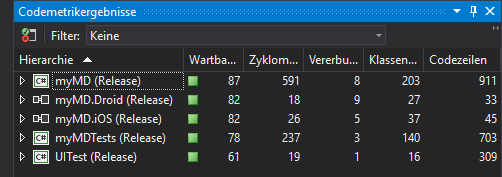
\includegraphics[scale=0.8]{graphics/Codemetrik_App}
\caption{Berechnete Codemetriken von VisualStudio}
\end{figure}

\printnoidxglossaries

% Abbildungsverzeichnis
\listoffigures
 
\end{document}